\newpage
\section{Eksamensopgave 4 - Ellære}
\subsection{Beregn erstatningsresistansen i resistorkoblingen}
Når man beregner erstatningsresistansen i en resistorkobling, ønsker man at finde én enkelt resistor, som kan erstatte hele koblingen og have samme samlede modstand. Kan man starte med at finde de resistorer der sidder i parallelforbindelsen, og beregne deres erstatningsresistansen. 
I denne opgave skal i beregne modstanden for en parallel forbindelse som også har en serie forbindelse. Dog inden man gør det angiver man hvad man vil kalde ens modstande for ikke at der bilver forvirrene.\newline
\begin{figure}[h!]
    \centering
    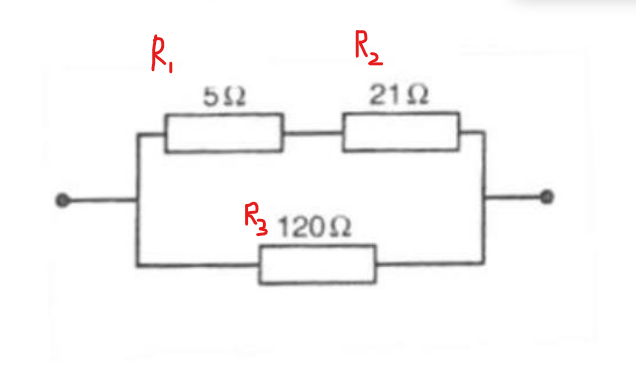
\includegraphics[width=0.5\textwidth]{figures/resistans.png}
    \caption{Indtegning af navne samt resistorkobling}
\end{figure}
\newline
Herefter skal man finde frem til værdien for den samlede erstatningsresistansen, da der er en serieforbindelse skal vi først beregne den samlede modstand af den før vi kan beregne parallelforbindelsen.
\begin{equation*}
    R_{12}=R_{1}+R_{2}
\end{equation*}
\begin{equation*}
   R=5\Omega+21\Omega=\mathcolorbox{yellow}{26\Omega}
\end{equation*}
Da de er parallel skal man huske at tage den reciprokke værdi til sidst. For at beregne den samlede modstand af en parallelforbindelsen anvdendes følgende formel, som basseres på Kirshoffs 1. lov, det Kirshoffs første lov siger er at $I_{1} = I_2 + I_3$ Altså at strømmen der går gennem et knudepunkt er lig den strøm der går ud af knudepunktet.
\begin{equation*}
    \frac{1}{R_{total}}=\frac{1}{R_{1}}+\frac{1}{R_{2}}
\end{equation*}
\begin{equation*}
    R_{total}=\left(\frac{1}{26\Omega}+\frac{1}{120\Omega}\right)^{-1}
\end{equation*}

\begin{equation*}
    R_{total}=\mathcolorbox{yellow}{21,37\Omega}
\end{equation*}

\subsection{Modstanden på 5~$\Omega$ laves af en kobbertråd med længden 60m. Bestem trådens radius.}
For at beregne kobbertrådens radius kan vi bruge følgende formel:
\begin{equation*}
    R=\rho\cdot\frac{l}{A}
\end{equation*}
R = Modstand i ohm ~$\left[ \Omega \right]$\newline
    $\rho$ = Resistivitet for kobbertråden er den på $0,0155 \cdot 10^{-6} \Omega$ \newline
    $l$ = Længden af kobbertråden\newline
    $A$ = Tværsnitsarealet\newline

For at bruge denne formel skal vi have isoleret A, som vi gør ved at gange med A på begge sider og derefter dividere med R på begge sider. Derfor kommer formlen til at se sådan ud.
\begin{equation*}
    A=\frac{l\cdot\rho}{R}
\end{equation*}
Nu kan vi indsætte vores værdier
\begin{equation*}
    A=\frac{60m\cdot0,0155 \cdot 10^{-6} \Omega \cdot m}{5\Omega}
\end{equation*}
\begin{equation*}
    A = \frac{9,3 \cdot 10^{-7} \cdot \Omega \cdot m^{2}}{5 \Omega} = 1,86 \cdot 10^{-7} \cdot m^{2} \approx 0,186 \cdot mm^{2}
\end{equation*}
Nu har vi arealet af en cirkel som betyder at vi kan bruge bruge formlen for arealet af en cirkel og isolere radiussen ved at dividere med ~$\pi$ på begge sider.
\begin{equation*}
    A=\pi*r^{2}
\end{equation*}
\begin{equation*}
    \frac{A}{\pi}=r^{2}
\end{equation*}
\begin{equation*}
    r^{2}=\frac{A}{\pi}
\end{equation*}
Nu når radiussen er blevet isoleret skal gøre så radius ikke er opløftet med 2 ved at tage kvadratroden på begge sider.
\begin{equation*}
    r=\sqrt{\frac{A}{\pi}}
\end{equation*}
Med den isolerede formel kan værderiene indsættes for at finde radiussen.
\begin{equation*}
    r=\sqrt{\frac{0,186mm^{2}}{\pi}} = \mathcolorbox{yellow}{0,243 mm}
\end{equation*}
\newpage
\subsection{Et batteri med hvilespændingen 1,4V og en indre modstand på 0,5~$\Omega$ tilsluttes resistorkoblingen. Skitser situationen og beregn polspændingen.}
\begin{figure}[h!]
    \centering
    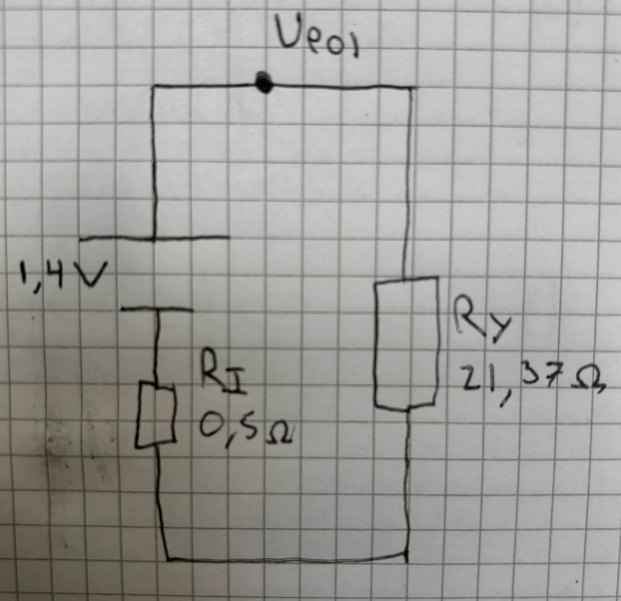
\includegraphics[width=0.5\textwidth]{figures/ellareskitse.png}
    \caption{Skitse af situationen}
\end{figure}
\begin{figure}[h!]
    \centering
    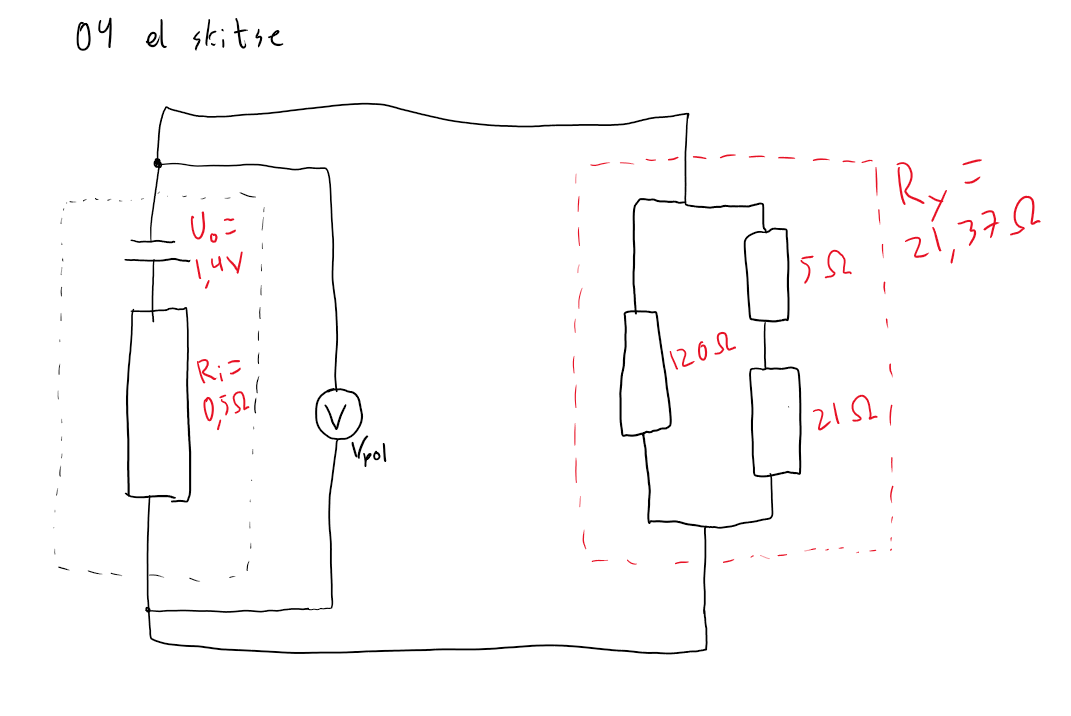
\includegraphics[width=0.8\textwidth]{figures/ellareskitseBille.png}
    \caption{Skitse af situationen, forbedret. Cirklen med V i er et voltmeter/spændingens måler og viser $U_{pol}$.}
\end{figure}
For at beregne polspændingen skal vi først have en formel.\newline
Først starter vi med Ohms low, hvor U er spændingen, R er modstanden og I er strømmen.
\begin{equation*}
    U = R \cdot I
\end{equation*}
Det betyder vi kender spændingen over de to modstande
\begin{equation*}
    U_{indre} = R_{Indre} \cdot I
\end{equation*}
\begin{equation*}
    U_{Ydre} = R_{Ydre} \cdot I
\end{equation*}
Derefter defineres $U_{Hvile}$ som er spændingen over batteriet når der ikke løber strøm igennem. Og det er summen af de to spændinger, som er den samlede spændingsforskel over batteriet.
\begin{equation*}
    U_{Hvile} = U_{Indre} + U_{Ydre}
\end{equation*}
Så kan man sætte ohms lov ind i formlen for $U_{Indre}$ og $U_{Ydre}$ til at blive til $R_{Indre} \cdot I$ og $R_{Ydre} \cdot I$.
\begin{equation*}
    U_{Hvile} = R_{Indre} \cdot I + R_{Ydre} \cdot I
\end{equation*}
Her bliver der introduceret en ny variabel $U_{pol}$, som kommer fra at $R_{Ydre} \cdot I$ er blevet forkortet til $U_{pol}$.
\begin{equation*}
    U_{Hvile} = R_{Indre} \cdot I + U_{pol}
\end{equation*}
Nu bliver $U_{pol}$ isoleret ved at minusse med $R_{Indre} \cdot I$ på begge sider hvor vi så til sidst får vores formel.
\begin{equation*}
    U_{pol}=U_{Hvile}-I\cdot R_{Indre}
\end{equation*}
Men før vi kan bruge formlen mangler vi at finde strømstyrken I. For at beregne den kan vi kigge på ohms lov som hedder $U = R \cdot I$. For at få I til at stå alene skal vi dividere med R på begge sider og bliver derfor til $I = \frac{U}{R}$
\begin{equation*}
    I_{total}=\frac{1,4V}{21,37\Omega+0,5\Omega}=0,064A
\end{equation*}
Når vi så har alle vores værdier kan vi indsætte dem ind i den første formel for så at beregne polspændingen.
\begin{equation*}
    U_{pol}=1,4V-0,5\Omega\cdot 0,064A=1,368V
\end{equation*}
\newpage